%Version 3.1 December 2024
% See section 11 of the User Manual for version history
%
%%%%%%%%%%%%%%%%%%%%%%%%%%%%%%%%%%%%%%%%%%%%%%%%%%%%%%%%%%%%%%%%%%%%%%
%%                                                                 %%
%% Please do not use \input{...} to include other tex files.       %%
%% Submit your LaTeX manuscript as one .tex document.              %%
%%                                                                 %%
%% All additional figures and files should be attached             %%
%% separately and not embedded in the \TeX\ document itself.       %%
%%                                                                 %%
%%%%%%%%%%%%%%%%%%%%%%%%%%%%%%%%%%%%%%%%%%%%%%%%%%%%%%%%%%%%%%%%%%%%%

%%\documentclass[referee,sn-basic]{sn-jnl}% referee option is meant for double line spacing

%%=======================================================%%
%% to print line numbers in the margin use lineno option %%
%%=======================================================%%

%%\documentclass[lineno,pdflatex,sn-basic]{sn-jnl}% Basic Springer Nature Reference Style/Chemistry Reference Style

%%=========================================================================================%%
%% the documentclass is set to pdflatex as default. You can delete it if not appropriate.  %%
%%=========================================================================================%%

%%\documentclass[sn-basic]{sn-jnl}% Basic Springer Nature Reference Style/Chemistry Reference Style

%%Note: the following reference styles support Namedate and Numbered referencing. By default the style follows the most common style. To switch between the options you can add or remove �Numbered� in the optional parenthesis. 
%%The option is available for: sn-basic.bst, sn-chicago.bst%  
 
%%\documentclass[pdflatex,sn-nature]{sn-jnl}% Style for submissions to Nature Portfolio journals
%%\documentclass[pdflatex,sn-basic]{sn-jnl}% Basic Springer Nature Reference Style/Chemistry Reference Style
\documentclass[pdflatex,sn-mathphys-num]{sn-jnl}% Math and Physical Sciences Numbered Reference Style
%%\documentclass[pdflatex,sn-mathphys-ay]{sn-jnl}% Math and Physical Sciences Author Year Reference Style
%%\documentclass[pdflatex,sn-aps]{sn-jnl}% American Physical Society (APS) Reference Style
%%\documentclass[pdflatex,sn-vancouver-num]{sn-jnl}% Vancouver Numbered Reference Style
%%\documentclass[pdflatex,sn-vancouver-ay]{sn-jnl}% Vancouver Author Year Reference Style
%%\documentclass[pdflatex,sn-apa]{sn-jnl}% APA Reference Style
%%\documentclass[pdflatex,sn-chicago]{sn-jnl}% Chicago-based Humanities Reference Style

%%%% Standard Packages
%%<additional latex packages if required can be included here>

\usepackage{graphicx}%
\usepackage{multirow}%
\usepackage{amsmath,amssymb,amsfonts}%
\usepackage{amsthm}%
\usepackage{mathrsfs}%
\usepackage[title]{appendix}%
\usepackage{xcolor}%
\usepackage{textcomp}%
\usepackage{manyfoot}%
\usepackage{booktabs}%
\usepackage{algorithm}%
\usepackage{algorithmicx}%
\usepackage{algpseudocode}%
\usepackage{listings}%
\usepackage{caption} % 추가
\usepackage{subcaption} % 추가

%%%%

%%%%%=============================================================================%%%%
%%%%  Remarks: This template is provided to aid authors with the preparation
%%%%  of original research articles intended for submission to journals published 
%%%%  by Springer Nature. The guidance has been prepared in partnership with 
%%%%  production teams to conform to Springer Nature technical requirements. 
%%%%  Editorial and presentation requirements differ among journal portfolios and 
%%%%  research disciplines. You may find sections in this template are irrelevant 
%%%%  to your work and are empowered to omit any such section if allowed by the 
%%%%  journal you intend to submit to. The submission guidelines and policies 
%%%%  of the journal take precedence. A detailed User Manual is available in the 
%%%%  template package for technical guidance.
%%%%%=============================================================================%%%%

%% as per the requirement new theorem styles can be included as shown below
\theoremstyle{thmstyleone}%
\newtheorem{theorem}{Theorem}%  meant for continuous numbers
%%\newtheorem{theorem}{Theorem}[section]% meant for sectionwise numbers
%% optional argument [theorem] produces theorem numbering sequence instead of independent numbers for Proposition
\newtheorem{proposition}[theorem]{Proposition}% 
%%\newtheorem{proposition}{Proposition}% to get separate numbers for theorem and proposition etc.

\theoremstyle{thmstyletwo}%
\newtheorem{example}{Example}%
\newtheorem{remark}{Remark}%

\theoremstyle{thmstylethree}%
\newtheorem{definition}{Definition}%

\raggedbottom
%%\unnumbered% uncomment this for unnumbered level heads

\begin{document}

\title[Article Title]{Calculating Ground-State-Energy of \(\mathrm{LiCoO_2}\) by using Fragment molecular orbital-based Variational Quantum Eigensolver}

%%=============================================================%%
%% GivenName	-> \fnm{Joergen W.}
%% Particle	-> \spfx{van der} -> surname prefix
%% FamilyName	-> \sur{Ploeg}
%% Suffix	-> \sfx{IV}
%% \author*[1,2]{\fnm{Joergen W.} \spfx{van der} \sur{Ploeg} 
%%  \sfx{IV}}\email{iauthor@gmail.com}
%%=============================================================%%

\author*[1]{\fnm{Choi} \sur{Yoonho}}\email{cyh195535@hanyang.ac.kr}

\author[1]{\fnm{Kim} \sur{Doyeon}}\email{cyh195535@hanyang.ac.kr}
\equalcont{These authors contributed equally to this work.}

\author[1]{\fnm{Kim} \sur{Doha}}\email{cyh195535@hanyang.ac.kr}

\author[1,2]{\fnm{Kwon} \sur{Younghun}}\email{cyh195535@hanyang.ac.kr}
\equalcont{These authors contributed equally to this work.}


\affil*[1]{\orgdiv{Department of applied Phisics}, \orgname{Hanyang University}, \orgaddress{\city{Ansan}, \postcode{15588}, \state{Republic of Korea}}}

\affil[2]{\orgdiv{Department of Intelligence, Information, and Quantum}, \orgname{Hanyang University}, \orgaddress{\city{Ansan}, \postcode{15588}, \state{Republic of Korea}}}


%%==================================%%
%% Sample for unstructured abstract %%
%%==================================%%

\abstract{The Variational Quantum Eigensolver (VQE) is a quantum algorithm designed to compute the ground-state energy of systems, and it holds significant promise for applications in areas like material science, drug discovery, and battery technology. However, the limited number of qubits available on current quantum computers makes it challenging to apply VQE to large, complex molecules in industrial set-tings. To address this limitation, we propose the use of the FMO-VQE approach to solve real-world problems. The Fragment Molecular Orbital (FMO) method breaks a system into smaller fragments for more manageable processing. Although previous work [1] has explored the FMO method within the VQE framework, it has been ap-plied only to hydrogen clusters, limiting its effectiveness to simpler cases. In this study, we assess the FMO-VQE approach in a more complex context, considering \(\mathrm{LiCoO_2}\), a material used as a cathode in lithium-ion batteries. We use the FMO-VQE method to calculate the ground-state energy of \(\mathrm{LiCoO_2}\), demonstrating its feasibility for more complex systems. This approach reduces the required qubit count from 24 to a maximum of 14, while maintaining accuracy comparable to classical methods. This reduction in qubits is crucial for the practical application of near-term quantum com-puters (NISQ). Our findings indicate that the FMO-VQE algorithm can overcome size-related limitations, making it feasible to apply VQE to larger molecular systems, thus paving the way for advancements in fields like battery technology and drug discovery.}

%%================================%%
%% Sample for structured abstract %%
%%================================%%

% \abstract{\textbf{Purpose:} The abstract serves both as a general introduction to the topic and as a brief, non-technical summary of the main results and their implications. The abstract must not include subheadings (unless expressly permitted in the journal's Instructions to Authors), equations or citations. As a guide the abstract should not exceed 200 words. Most journals do not set a hard limit however authors are advised to check the author instructions for the journal they are submitting to.
% 
% \textbf{Methods:} The abstract serves both as a general introduction to the topic and as a brief, non-technical summary of the main results and their implications. The abstract must not include subheadings (unless expressly permitted in the journal's Instructions to Authors), equations or citations. As a guide the abstract should not exceed 200 words. Most journals do not set a hard limit however authors are advised to check the author instructions for the journal they are submitting to.
% 
% \textbf{Results:} The abstract serves both as a general introduction to the topic and as a brief, non-technical summary of the main results and their implications. The abstract must not include subheadings (unless expressly permitted in the journal's Instructions to Authors), equations or citations. As a guide the abstract should not exceed 200 words. Most journals do not set a hard limit however authors are advised to check the author instructions for the journal they are submitting to.
% 
% \textbf{Conclusion:} The abstract serves both as a general introduction to the topic and as a brief, non-technical summary of the main results and their implications. The abstract must not include subheadings (unless expressly permitted in the journal's Instructions to Authors), equations or citations. As a guide the abstract should not exceed 200 words. Most journals do not set a hard limit however authors are advised to check the author instructions for the journal they are submitting to.}

\keywords{VQE, Quantum Computing, Lithium-ion batteries}


%%\pacs[JEL Classification]{D8, H51}

%%\pacs[MSC Classification]{35A01, 65L10, 65L12, 65L20, 65L70}

\maketitle

\section{Introduction}\label{sec1}

The ground state and energy of a molecule are fundamental to understanding molecular bonds and their structural properties. 
This information is essential across a wide range of chemical research areas, including the development of new drugs [2-4], materials [5, 6], and advanced cathode materials for secondary batteries [7, 8]. 
Currently, classical computers are used to calculate the ground-state energy of molecules [9-11].
However, as the number of atoms in a molecule increases, or as the atomic number of the elements involved grows, the complexity of the system also increases exponentially.
This results in a rapid rise in the number of particles and their interac-tions, which are represented in the molecule’s Hamiltonian. 
The need to process these interactions requires significant computational resources and memory. 
Consequently, calculating the ground-state energy of large molecules becomes increasingly challeng-ing on classical computers.

Quantum computers, which are an emerging technology, offer a promising alterna-tive. Unlike classical computers, quantum computers use qubits, having superposi-tions of  0 and 1 states. 
This allows quantum computers to potentially calculate the ground-state energy of a molecule much more efficiently. 
While classical computers require exponential increases in memory as the system size grows, quantum comput-ers only need a polynomial increase in qubits to handle the same task. 
This enables quantum computers to process large molecules that would be infeasible for classical computers.
One approach to calculating the ground-state energy of a molecule on a quantum computer is the Quantum Phase Estimation (QPE) algorithm, which determines the eigenvalues and eigenstates of a unitary matrix [12-16]. 
However, QPE is highly accurate but requires a large number of qubits, which makes it impractical for current quantum devices, particularly noisy intermediate-scale quantum (NISQ) devices [17]. 
These devices are limited by noise, lack of precision, and a relatively small number of qubits, making it difficult to implement QPE effectively.

The Variational Quantum Eigensolver (VQE) is another algorithm designed to solve eigenvalue problems on NISQ-level quantum computers by combining both quantum and classical computing [18-21].
VQE uses a variational approach to construct a parameterized trial wavefunction, which is iteratively adjusted until it con-verges to provide an upper bound for the ground-state energy. 
The quantum computer performs the expectation value calculations, while the classical computer optimizes the trial wavefunction’s parameters.
Unlike QPE, VQE requires fewer qubits and allows for the optimization process to be handled by a classical computer, 
making it a promising candidate for commercial quantum computing applications in the NISQ era. 
Despite its potential, current quantum computers still face significant challenges, including errors and decreased accuracy as circuit depth increases. 
Additionally, the limited number of available qubits restricts the ability to calculate the ground-state energy of very large molecules. 
To address these issues, one promising approach is the Fragment Molecular Orbital-based Variational Quantum Eigensolver (FMO-VQE).
Initially proposed by Lim et al. [1], the FMO-VQE method applies the classical FMO technique, which divides a molecule into smaller fragments and calculates the ground-state energy for individual monomers and dimers [22-25]. 
These results are then used to estimate the total ground-state energy of the entire molecule. 
While Lim et al. demonstrated the FMO-VQE method on hydrogen clusters, its application to more complex molecules remain unexplored. 
This raises the question of whether the FMO-VQE approach is effective for real-world applications. 
In this study, we investi-gate the performance of FMO-VQE by considering \(\mathrm{LiCoO_2}\), a key material used as a cathode in lithium-ion batteries. We calculate the ground-state energy of \(\mathrm{LiCoO_2}\) and compare the results with those from classical computations, demonstrating the poten-tial of FMO-VQE for handling complex materials like \(\mathrm{LiCoO_2}\).

\section{Methods}\label{sec2}

\subsection{Lithium-ion battery}\label{subsec2.1}
Lithium-ion batteries are widely used secondary batteries in various industries. A lithium-ion battery consists of an anode material, a cathode material, and an electrolyte, with lithium oxide typically used as the cathode material. This compound has a layered structure of CoO₂⁻ oxide, with \(\mathrm{Li^+}\) ions bonded between each layer. The ener-gy charge of the battery depends on the extent to which the lithium ions are oxidized in the oxide [1-3].
Lithium is known to have limited reserves in the world, prompting the need for sustainable solutions [4]. One such solution is to maximize the energy charged per lithium ion. This is critical both in terms of conserving lithium resources and for advanc-ing battery miniaturization[5, 6]. To calculate the amount of energy stored per lithium ion, it is essential to compute the ground state of the molecule. However, this calcu-lation is typically done using classical methods, and the ability to calculate larger molecules or more complex combinations is limited.
In this study, we demonstrate the application of the VQE algorithm to \(\mathrm{LiCoO_2}\) molecules and highlight the potential of quantum computers in the field of battery development.
\begin{figure}[H]
  \centering
  \begin{subfigure}[b]{0.45\textwidth}
    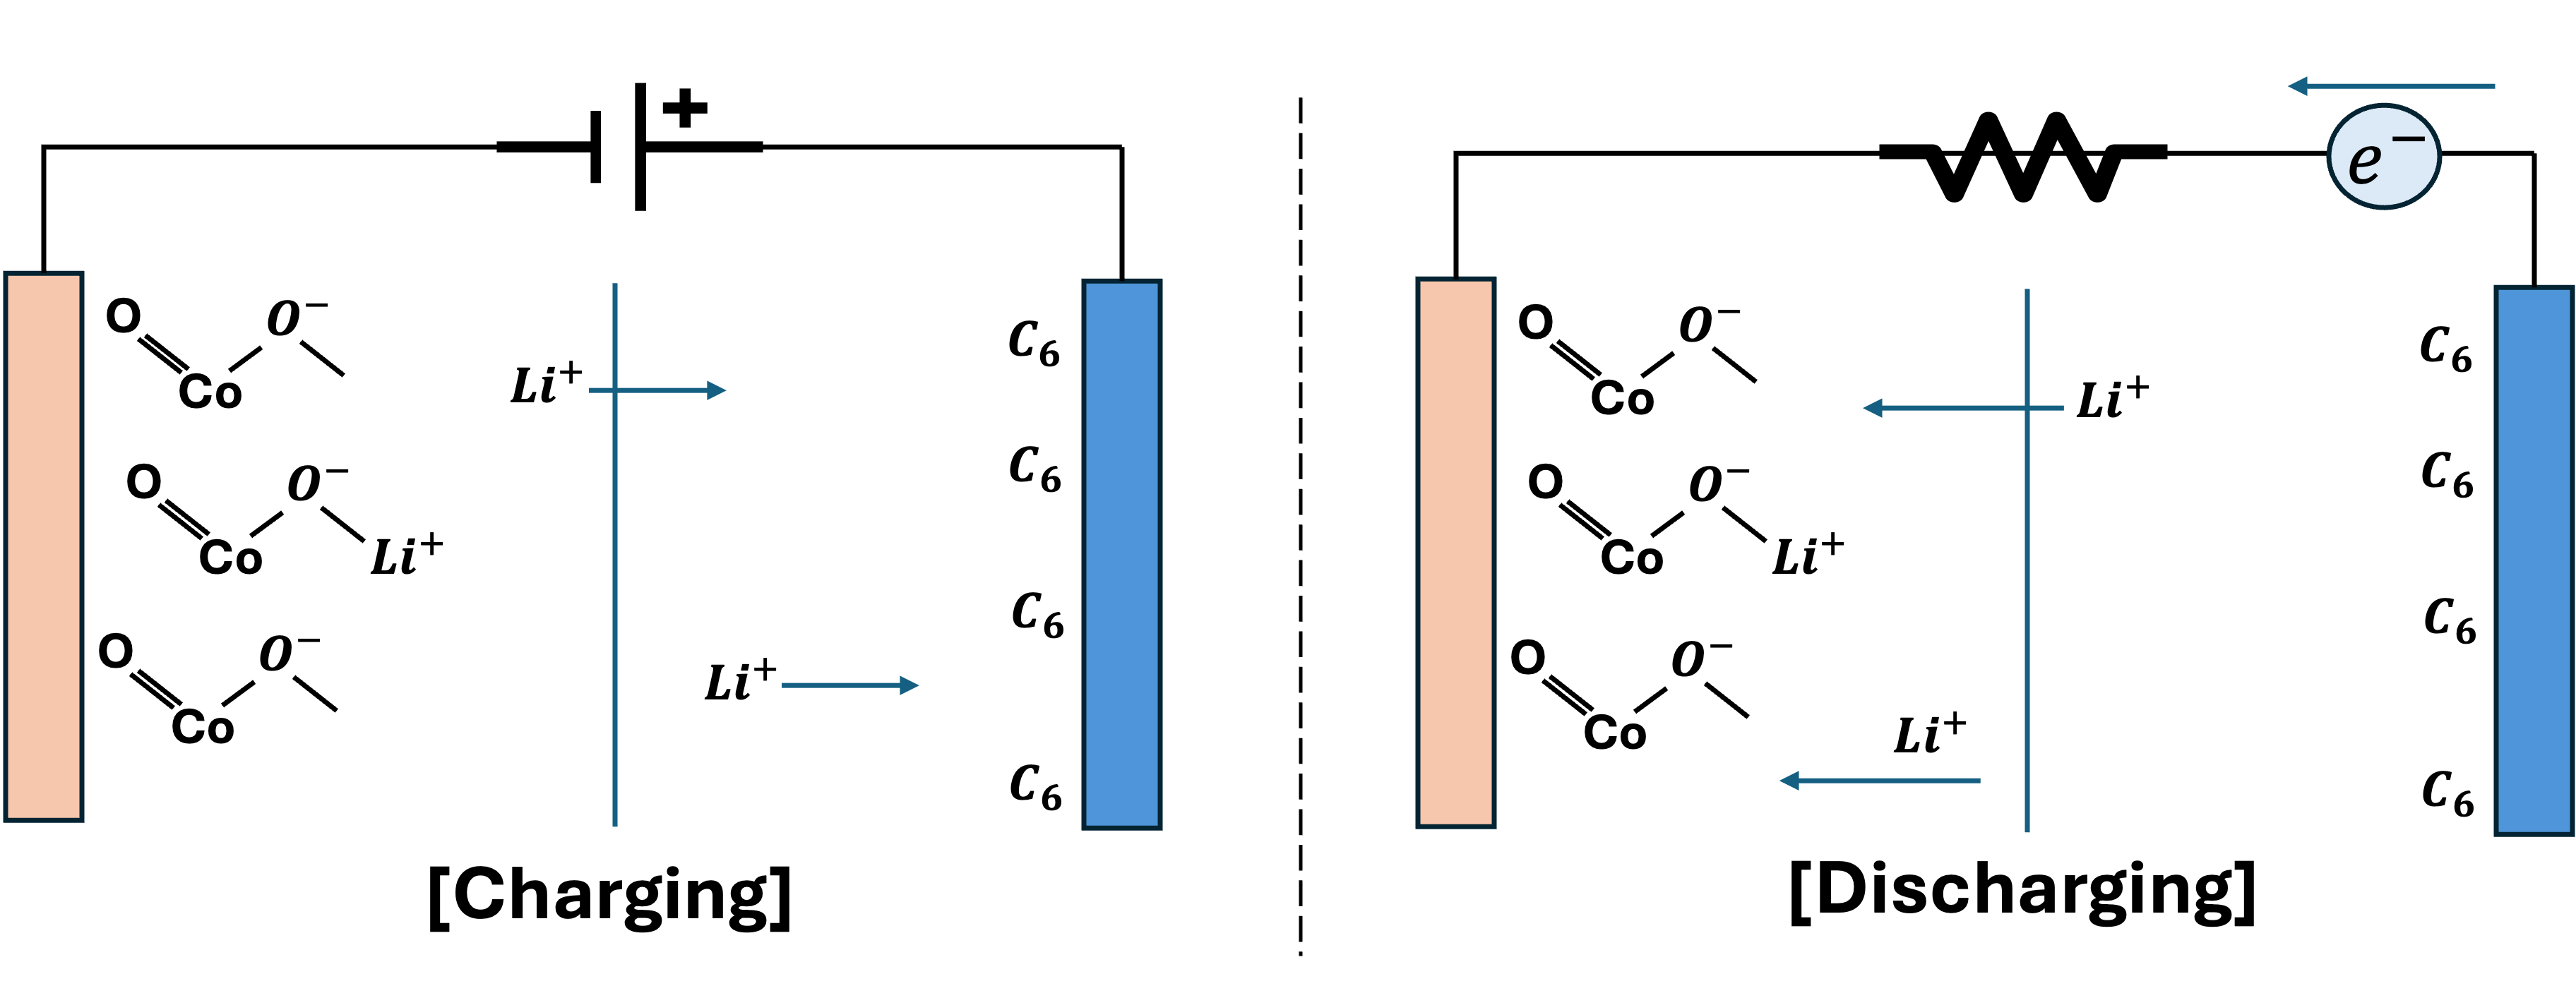
\includegraphics[width=\textwidth]{fig/Cha_discha.png}
    \caption{논문의 모식도}
    \label{fig:first}
  \end{subfigure}
  \hfill
  %\vrule width 1pt  % 수직선 추가 (굵기: 1pt)
  \hfill
  \begin{subfigure}[b]{0.45\textwidth}
    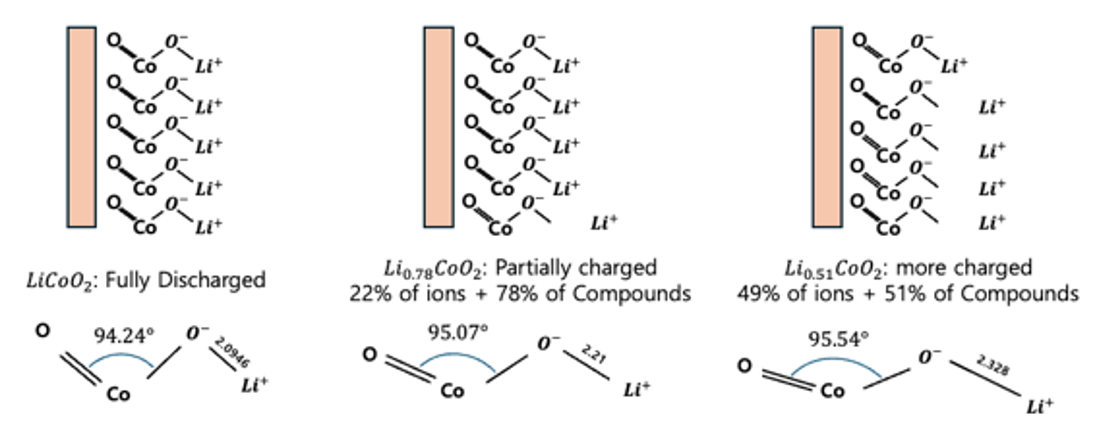
\includegraphics[width=\textwidth]{fig/char.png}
    \caption{내가정리}
    \label{fig:second}
  \end{subfigure}
  \caption{(a) a Schematic of battery charging and discharging. The red-colored elements represent the cathode, while the blue-colored elements represent the anode. The arrows represent the movement of lithium ions and electrons. (b) Depending on the oxidation state (denoted as x in \(\mathrm{Li_xCoO_2}\)) of each compound, the upper figure represents the relative number of lithium ions separated from the cathode, while the lower figure illustrates the average geometry of \(\mathrm{LiCoO_2}\).}
  \label{fig:two_figures_side_by_side}
\end{figure}
When a voltage is applied to the anode and cathode to supply electrons (i.e., during charging), the  \(\mathrm{Li^+}\) ions migrate to the anode. 
Upon discharging from this charged state, the \(\mathrm{Li^+}\) ions from the negative electrode recombine with the positive electrode, as shown in the Fig. 1 Left), and current flows through the resistor. 
During this pro-cess, depending on the oxidation state of lithium, the average geometry of the molecular structure changes, as illustrated in Fig. 1 Right).
Therefore, the energy stored in the bulk can be estimated using this geometry. 
The energy of the molecule is calculated by assuming a gas-phase model, which treats the average oxide structure as a single molecule.

\subsection{VQE(Variational Quantum Eigensolver)}\label{subsec2.2}
\begin{figure}[H]
\centering
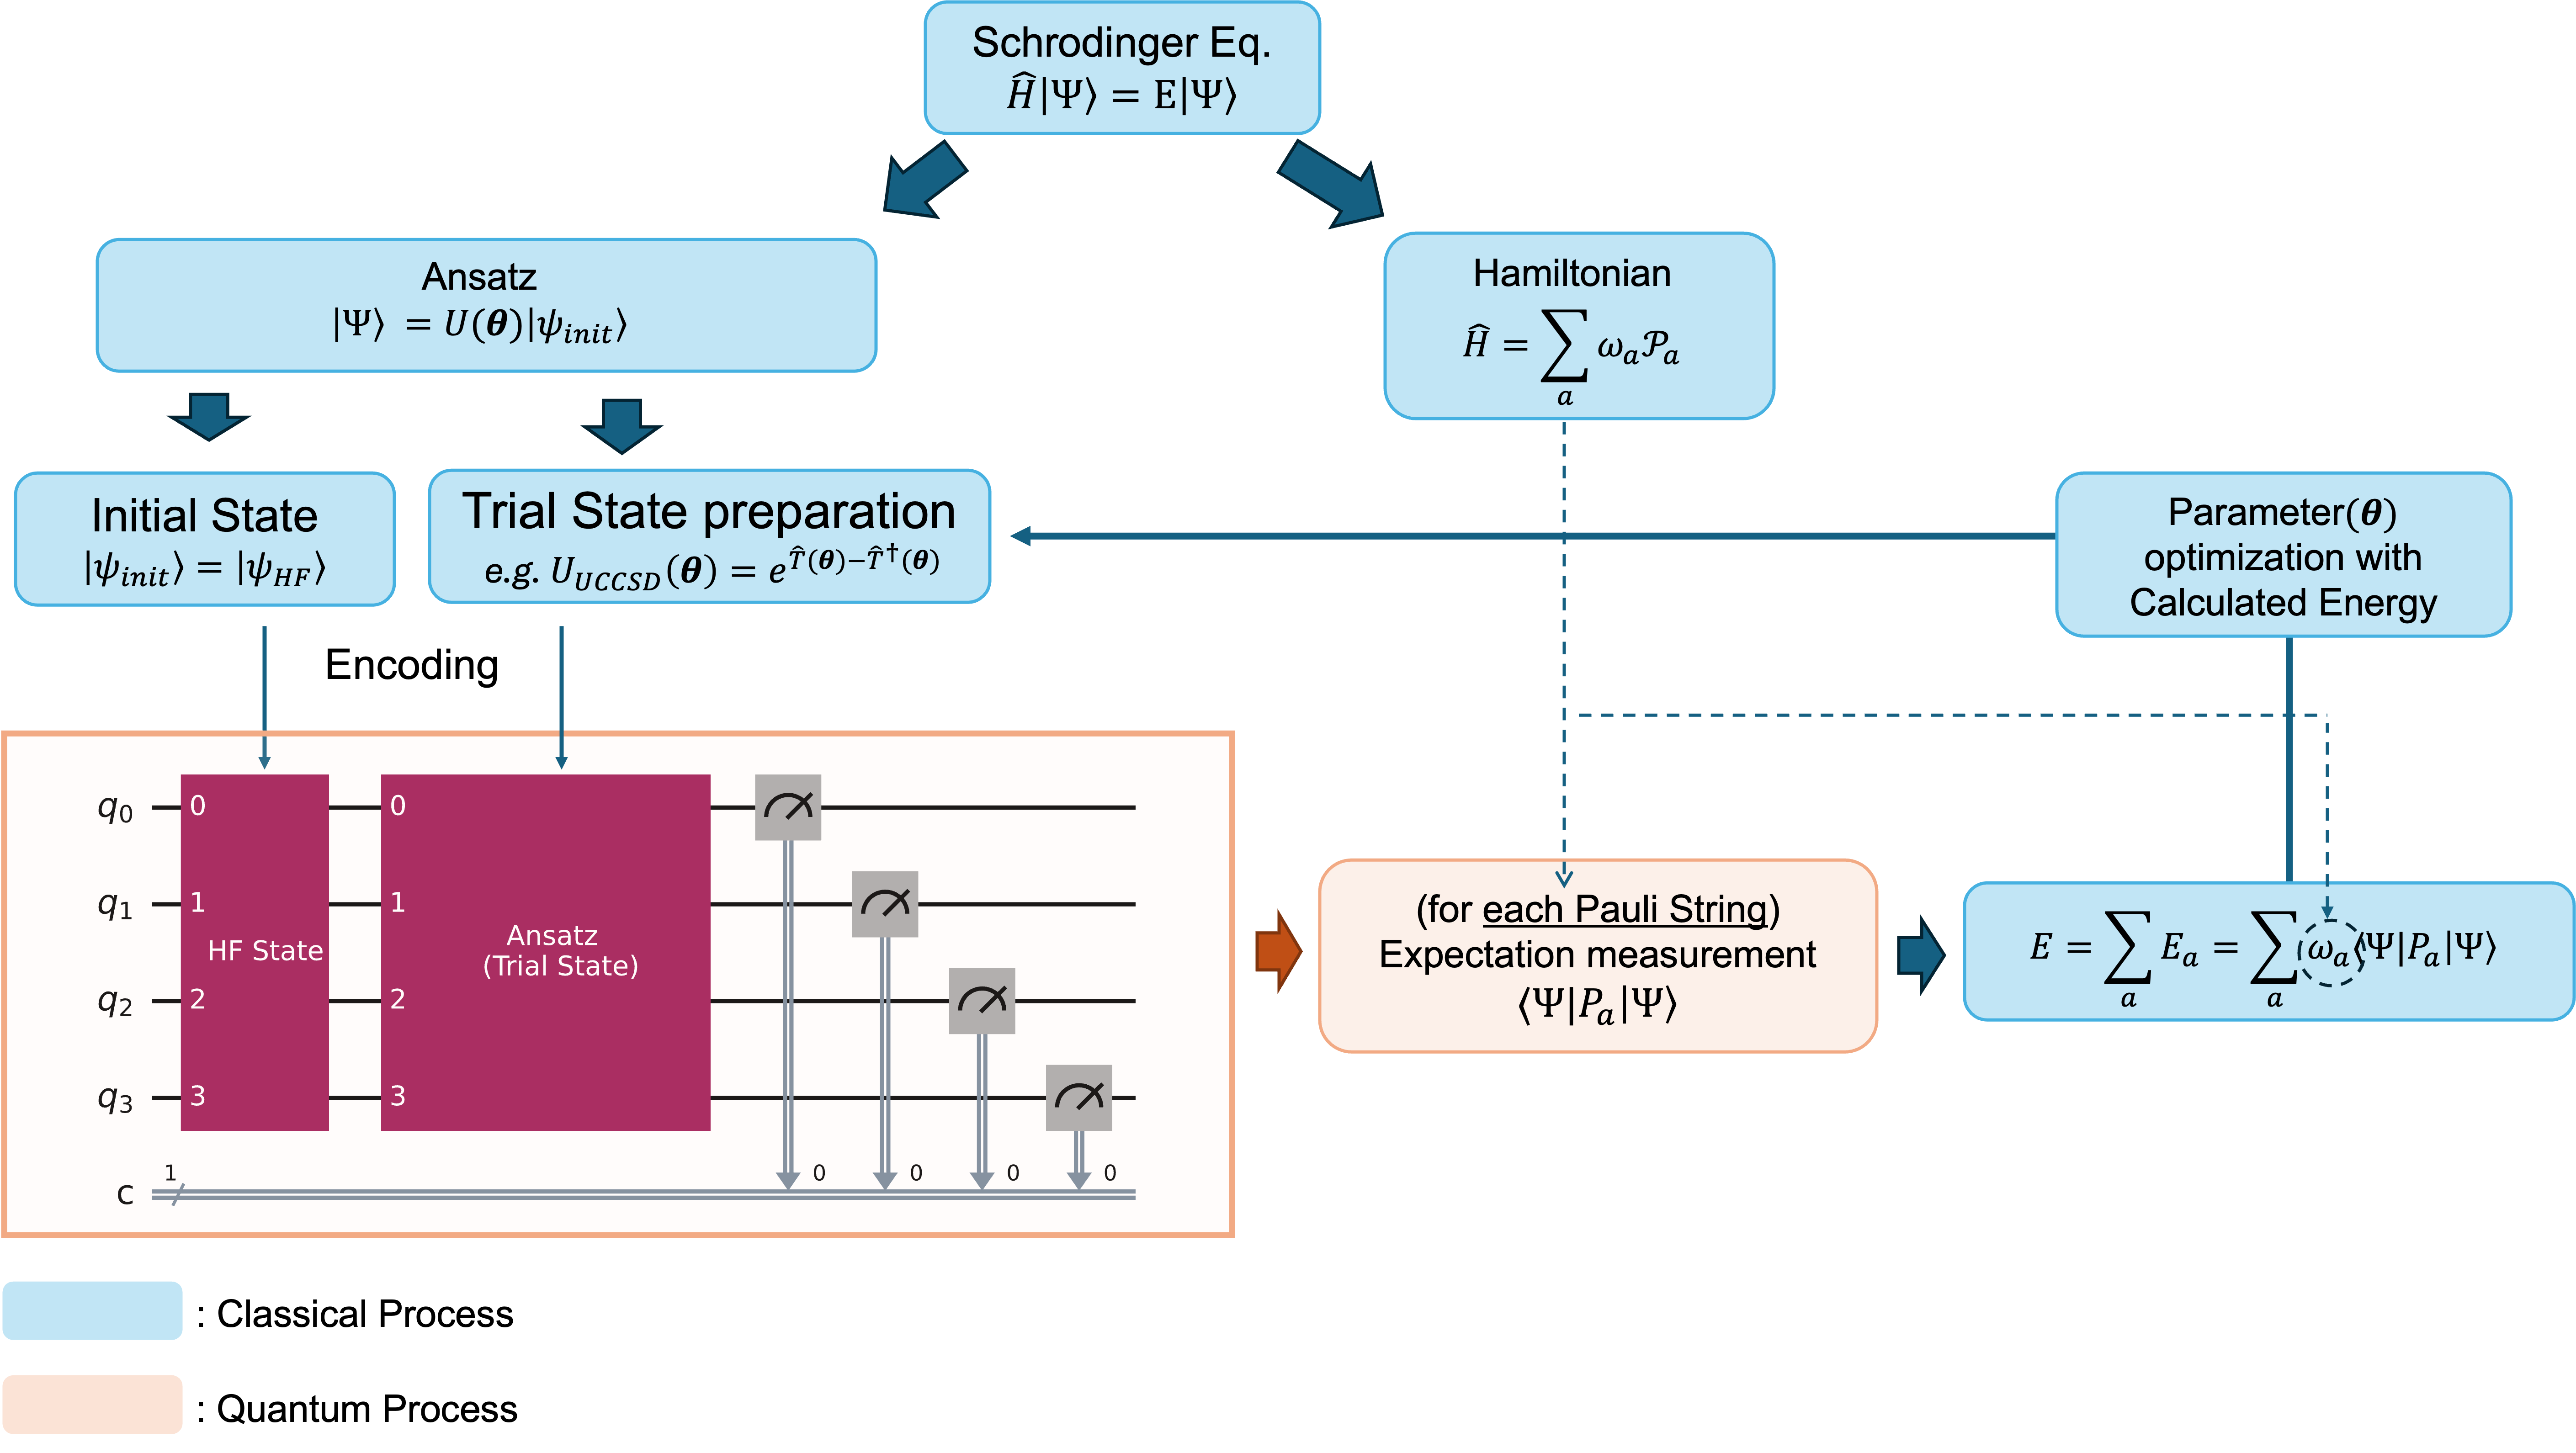
\includegraphics[width=0.8\textwidth]{fig/VQE_pipeline.png}
\caption{VQE Pipeline. Starting from the Schrödinger equation of the system, the process involves finding an appropriate measurement basis using the Hamiltonian, constructing an Ansatz to represent an arbitrary state with a parameterized quantum circuit, and finding the ground state energy through the variational method by performing measurements and updating the parameters}\label{Fig.2}
\end{figure}
The Variational Quantum Eigensolver (VQE) algorithm is an eigenvalue problem-solving method first proposed by Peruzzo et al [18]. It works by computing the ener-gy in Hilbert space, providing an upper bound on the ground state energy according to the variational principle. VQE calculates the ground state energy of a system by measuring the energy on a quantum computer and performing optimization on a clas-sical computer. To measure the energy of a system on a quantum computer, the Ham-iltonian must be mapped to a form that can be represented as a quantum circuit. Addi-tionally, an arbitrary quantum state needs to be encoded into the circuit for the meas-urement process.

\subsubsection{Hamiltonian}\label{subsec2.2.1}
The Hamiltonian of a molecule is represented by the Electronic Structure Hamiltonian as follows:
\begin{align}
\hat{H}_{el} 
&= \sum_{i} \frac{\nabla_{\mathbf{r}_i}^2}{m_i}
+ \sum_{I} \sum_{i} \frac{Z_I e^2}{\left| \mathbf{R}_I - \mathbf{r}_i \right|}
+ \sum_{i} \sum_{j>i} \frac{e^2}{\left| \mathbf{r}_i - \mathbf{r}_j \right|}
\end{align}
where \(r_i\) denotes the position vector of the i-th electron, 
\(R_I\) denotes the position of the I-th nucleon, and \(Z_I\) is the atomic number of the I-th nucleon. 
To map this Hamiltonian to the Pauli gates, we express it in second quantized form using fermionic creation/annihilation operators [7-9], as follows:
\begin{align}
\hat{H} 
&= \sum_{p,q} h_{pq} \, \hat{a}_p^{\dagger} \hat{a}_q
+ \frac{1}{2} \sum_{p,q,r,s} h_{pqrs} \, \hat{a}_p^{\dagger} \hat{a}_q^{\dagger} \hat{a}_r \hat{a}_s
\end{align}
\begin{equation*}
\text{where,} \quad 
h_{pq} = \langle \phi_p \vert \hat{H}_{\mathrm{el}} \vert \phi_q \rangle, \quad
h_{pqrs} = \langle \phi_p \, \phi_q \vert \hat{H}_{\mathrm{el}} \vert \phi_r \, \phi_s \rangle
\end{equation*}
Fermionic operators can be mapped to Pauli gates using Jordan-Wigner mapping, Parity mapping, and bravyi-kitaev mapping [10, 11]. 
In this experiment, we will use the Parity mapping method. 
Parity mapping expresses the creation-annihilation operator through a Pauli gate by corresponding the parity of the i-th qubit to the parity of the electron occupancy of the i-th orbital. 
In this case, the parity of the \(\alpha-\) spin and \(\beta-\) spin of the molecule can be utilized to reduce the number of qubits required by two. 
The resulting Hamiltonian of the mapping is represented by a Pauli string \(P_a\) and its weights or linear coefficients \(\omega_a\) as shown below.
\begin{equation}
\hat{H} = \sum_{a} \omega_{a} \, \mathcal{P}_{a}
\end{equation}

\subsubsection{Ansatz}\label{subsec2.2.2}
To represent arbitrary quantum states, we construct a parameterized quantum circuit (PQC) with linear coefficients corresponding to each basis as parameters. The perfor-mance of the ansatz is difficult to evaluate, and it is not known a priori which ansatz is better for different systems. Therefore, in this experiment, we use two different ansatzes to achieve better results.

\paragraph{Two-local(Efficient SU2) Ansatz} \leavevmode \newline
The quantum state of a single qubit is represented by a rotation gate with two arbitrary angles on the Bloch sphere. 
If the angle of the rotation gate is treated as a parameter, and the entanglement — a property of qubits in a multi-qubit system — is expressed using a CNOT gate, 
then the quantum state of an arbitrary multi-qubit system can be expressed using these parameters.
\begin{figure}[H]
\centering
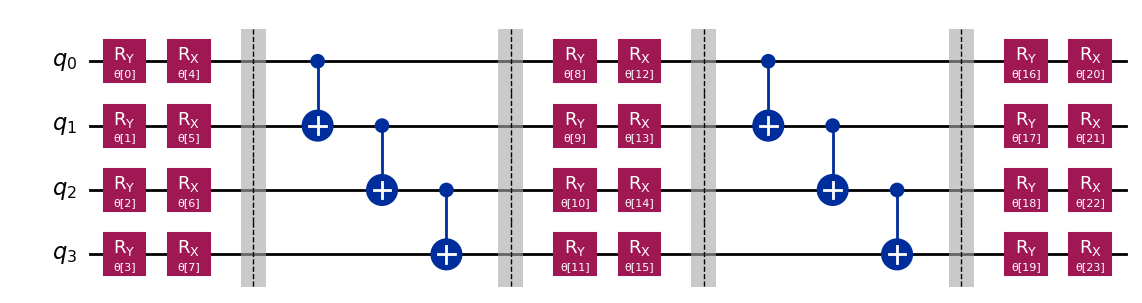
\includegraphics[width=0.8\textwidth]{fig/twolocal.png}
\caption{An example of a Two-Local Ansatz for a 4-Qubit system with 2 repetitions. The regions represented by dashed lines and the gray area distinguish the layers. The regions represent-ed by Rx and Ry gates, which include the parameter θ, represent the "rotation layer", while the regions represented by CNOT gates correspond to the "entanglement layer".}\label{Fig.3}
\end{figure}
The construction of the Two-Local Ansatz does not require an interpretation of the Hamiltonian. It is a representation of an arbitrary quantum state that is encoded in hardware, making it hardware-efficient.

\paragraph{UCCSD(Unitary Coupled Cluster Singles and Doubles) Ansatz} \leavevmode \newline
Through second quantization, we express the Hamiltonian operator in terms of the basis of the molecular orbitals of the system. Ultimately, the state we are looking for is represented in the same Hilbert space as the Hamiltonian. By using the same spin-orbitals as the basis, we can express any quantum state in the Hilbert space where the Hamiltonian exists. In this way, the quantum state is expressed through Coupled-Cluster Theory, using the spin-orbital wavefunctions of the molecule as the basis [12, 13]. When considering only second-order excitations, it is represented as a unitary operator, UCCSD (Unitary Coupled-Cluster Singles and Doubles), with the following expression[14]:
\begin{equation*}
\hat{T} = \hat{T}_1 + \hat{T}_2 \quad \text{(Cluster operator)}
\end{equation*}
\begin{equation*}
\text{where,} \quad 
\hat{T}_1 = \sum_{i,a} c_i^a \, \hat{a}_a^{\dagger} \hat{a}_i, \quad
\hat{T}_2 = \sum_{i,j,a,b} t_{ij}^{ab} \, \hat{a}_a^{\dagger} \hat{a}_b^{\dagger} \hat{a}_j \hat{a}_i
\end{equation*}
\begin{equation}
\vert \Psi \rangle_{\mathrm{UCCSD}} = e^{\left( \hat{T} - \hat{T}^{\dagger} \right)} \vert \psi_{\mathrm{ref}} \rangle
\end{equation}
The states are represented by creation and annihilation operators, which can be en-coded in quantum circuits using either Jordan-Wigner mapping or parity mapping. The energy of the system is calculated by measuring the expectation value for each Pauli string in the Hamiltonian within these quantum circuits. By iterating over these measurements and optimizing the parameters of the ansatz to minimize the calculated energy, an upper bound on the ground state energy is determined. The resulting min-imum corresponds to the ground state energy calculated by the VQE algorithm for the system.


\subsection{FMO (Fragmental Molecular orbital)}\label{subsec2.3}
\begin{figure}[H]
\centering
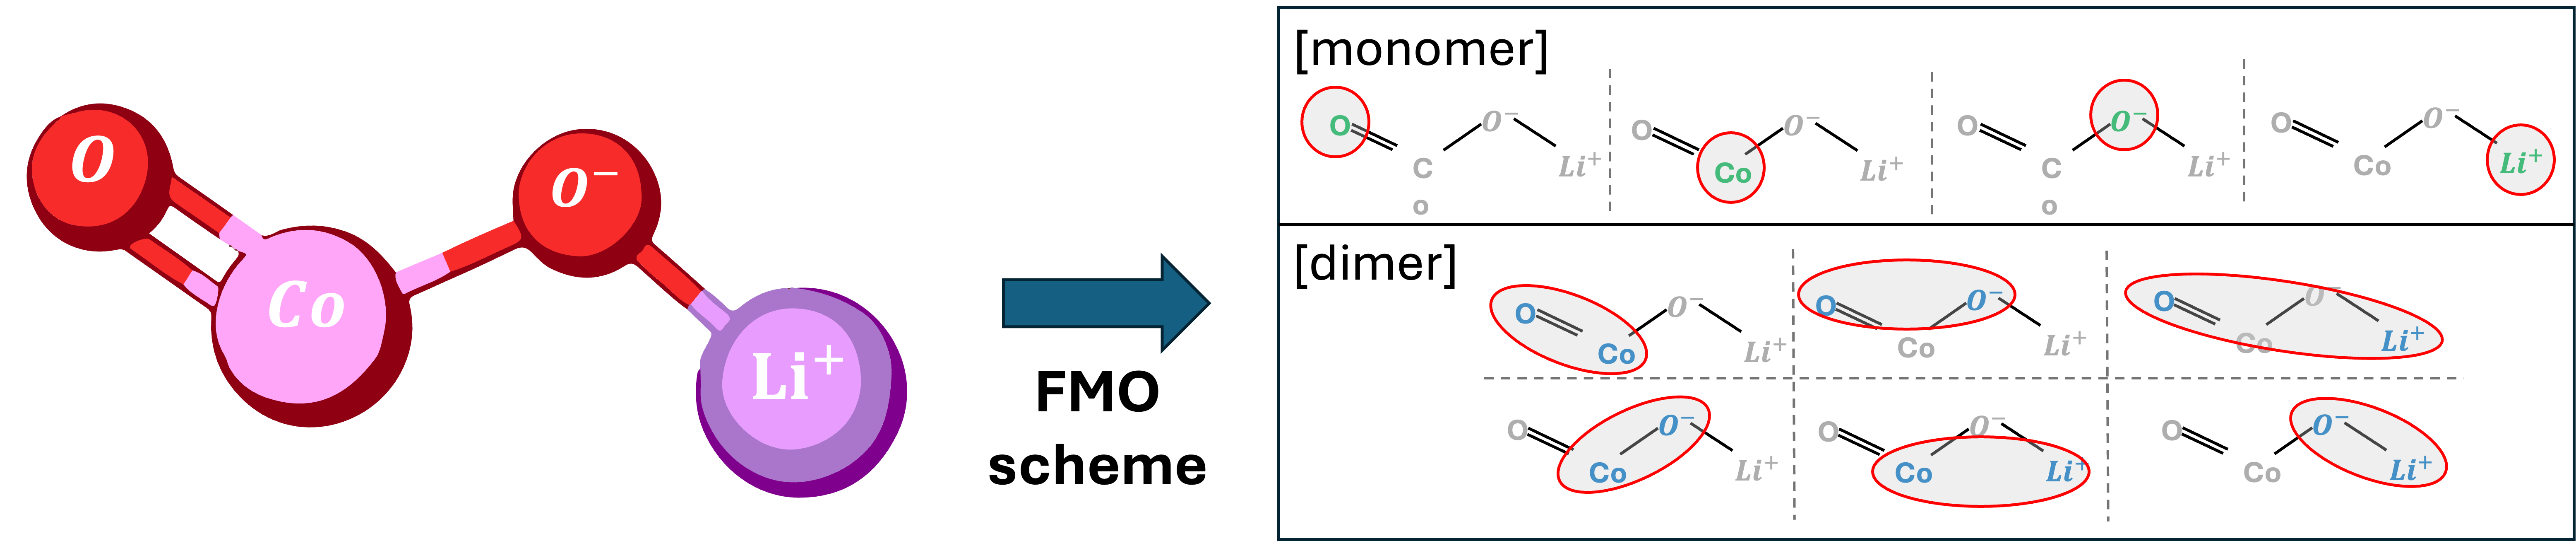
\includegraphics[width=0.8\textwidth]{fig/LiCoO2_FMO.png}
\caption{An example of the FMO scheme in \(\mathrm{LiCoO_2}\)}\label{Fig.4}
\end{figure}
The FMO method is a method that divides a whole molecular system into smaller system fragments and approximates the energy of the whole system by using the energy of one fragment (monomer) and the energy of pairs of fragments (dimers). When calculating the ground state energy of a molecule by the usual method, the computational complexity is exponential in the size of the system. However, the FMO method can effectively reduce the computational complexity by dividing a large system into parts. 
The FMO method has two main steps. The first is the FMO-based restricted Hartree-Fock (FMO-RHF) process, which calculates the RHF through the Hamiltonian of monomers and dimers. The Hamiltonian of monomer \(\mathrm{(\hat{H}_{A})}\) and the Hamiltonian of dimer\(\mathrm{(\hat{H}_{AB})}\) are as follows. 
\begin{equation}
\hat{H}_A = 
\sum_{i \in A} \Bigg[
    -\frac{\nabla_{\mathbf{r}_i}^2}{m_e}
    - \sum_I \frac{Z_I}{|\mathbf{r}_i - \mathbf{R}_I|}
    + \sum_{C \neq A}^{N_{\mathrm{tot}}} 
      \int d\mathbf{r}' \, \frac{\rho_J(\mathbf{r}')}{|\mathbf{r}_i - \mathbf{r}'|}
\Bigg]
+ \sum_{i \in A} \sum_{i<j \in A} \frac{1}{|\mathbf{r}_i - \mathbf{r}_j|}\label{eq5}
\end{equation}
\begin{equation}
\hat{H}_{AB} = 
\sum_{i \in A,B} \Bigg[
    -\frac{\nabla_{\mathbf{r}_i}^2}{m_e}
    - \sum_I \frac{Z_I}{|\mathbf{r}_i - \mathbf{R}_I|}
    + \sum_{C \neq A,B}^{N_{\mathrm{tot}}} 
      \int d\mathbf{r}' \, \frac{\rho_J(\mathbf{r}')}{|\mathbf{r}_i - \mathbf{r}'|}
\Bigg] + \sum_{i \in A,B} \sum_{i<j \in A,B} \frac{1}{|\mathbf{r}_i - \mathbf{r}_j|}
\end{equation}
(Where A,B are the respective fragments. C refers to the fragments that are not included in monomer A or dimer AB, and the term \(\rho_J(r')\) is the electric charge density of the fragments outside the monomer or dimer.) By calculating the RHF of each monomer and dimer through the Hamiltonian above, we can get \({E^\mathrm{FMO-RHF}}\), which can be expressed as follows.
\begin{equation}
E^{\mathrm{FMO2\!-\!RHF}} = E^{\mathrm{FMO1\!-\!RHF}} + \Delta E^{\mathrm{FMO2\!-\!RHF}}
\end{equation}
\begin{equation}
E^{\mathrm{FMO1\!-\!RHF}} = \sum_{A}^{N} E_A
\end{equation}
\begin{equation}
\Delta E^{\mathrm{FMO2\!-\!RHF}} = \sum_{A > B}^{N} \Big[ E_{IJ} - E_I - E_J \Big]
\end{equation}
In the above equations, N refers to all fragments. From the above equations, we can get the HF energy including the electrostatic potential of the whole molecule. The next step is to proceed with FMO based coupled-cluster (FMO-CC). This process is performed to obtain a more accurate value of the FMO-RHF energy, and since this process does not include the electrostatic potential, the Hamiltonian can be calculated using the Electronic Structure Hamiltonian defined earlier. The process of calculating the total energy \(E^\mathrm{FMO-CC}\) and correlation energy \(E^\mathrm{FMO-corr}\) obtained through FMO-CC is as follows.
\begin{equation}
E^{\mathrm{FMO}n\!-\!\mathrm{CC}} = E^{\mathrm{FMO}n\!-\!\mathrm{RHF}} + E^{\mathrm{FMO}n\!-\!\mathrm{corr}}
\end{equation}
\begin{equation}
E^{\mathrm{FMO2\!-\!corr}} = E^{\mathrm{FMO1\!-\!corr}} + \Delta E^{\mathrm{FMO2\!-\!corr}}
\end{equation}
\begin{equation}
E^{\mathrm{FMO1\!-\!corr}} = \sum_{A}^{N} E_A^{\mathrm{corr}}
\end{equation}
\begin{equation}
\Delta E^{\mathrm{FMO2\!-\!corr}} = \sum_{A>B}^{N} 
\left( E_{IJ}^{\mathrm{corr}} - E_I^{\mathrm{corr}} - E_J^{\mathrm{corr}} \right)
\end{equation}
In the above, the FMO-RHF and FMO-CC processes should be separated because the Hamiltonian used in the two processes may be different, and the FMO-CC process should proceed after the SCF calculation of FMO-RHF converges. However, in this experiment, the electrostatic potential term in the FMO-RHF Hamiltonian was approximated by ignoring it, so each process was carried out consecutively and the total energy was calculated from the obtained monomer and dimer energies as follows.

\subsection{FMO-VQE (Fragment molecular orbital-based Varational Quantum Eigensolver)}\label{subsec2.4}
\begin{figure}[H]
\centering
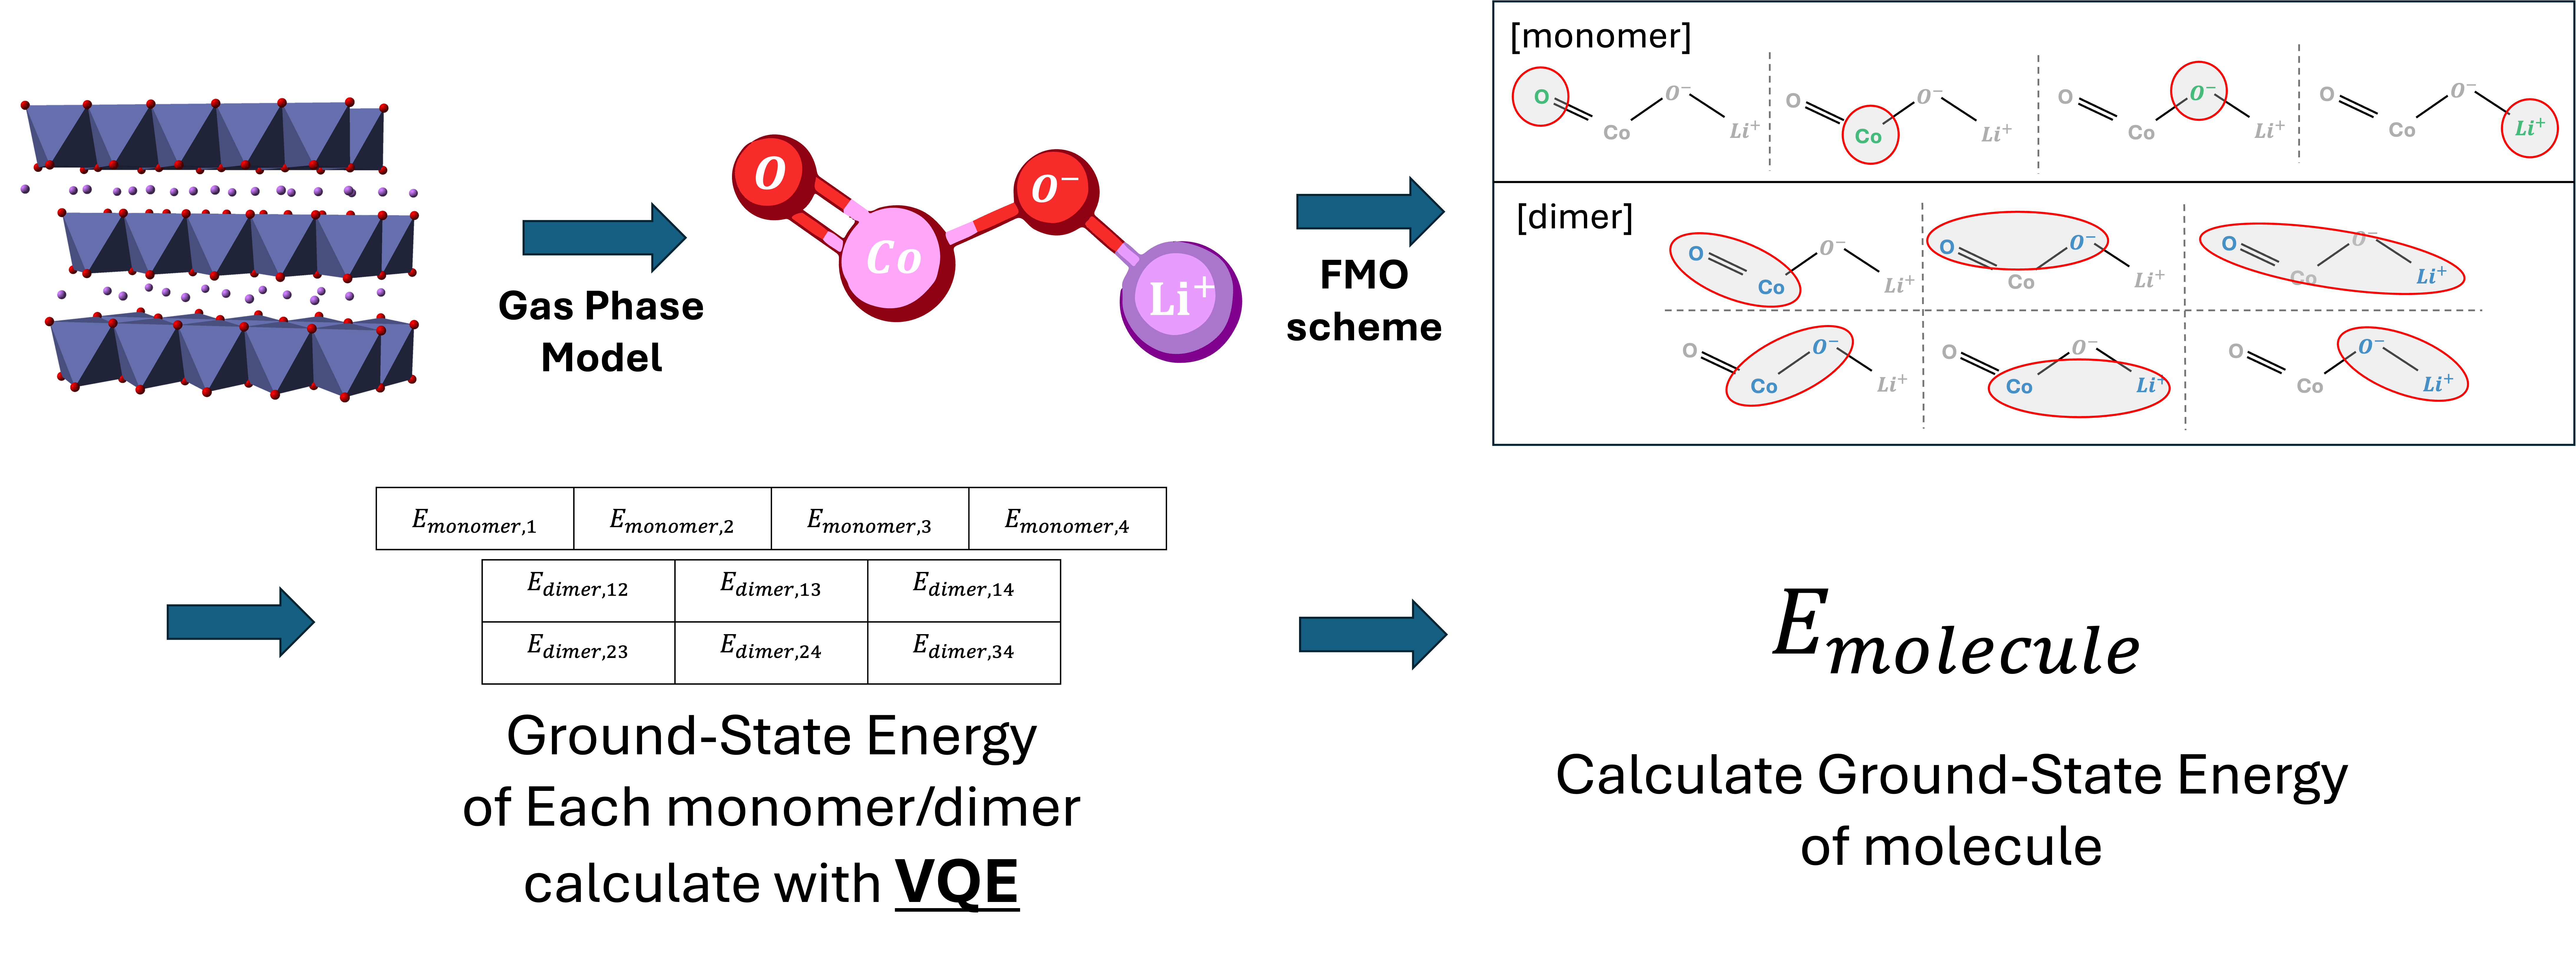
\includegraphics[width=0.8\textwidth]{fig/FMO_VQE_schme.png}
\caption{An illustration of applying the FMO/VQE method. 1) \(\mathrm{LiCoO_2}\) compound in the cathode material forms a layered structure, However, assuming a gas-phase model, it is considered that a single compound exists as a molecule. 2) The FMO scheme is applied to form monomers and dimers. 3) The ground state energy of each fragment is calculated using VQE. 4) The ground state energy of the entire molecule is then calculated using the energies of each fragment.}\label{Fig.5}
\end{figure}
FMO-VQE is an algorithm first introduced by Lim et al. that combines the VQE algorithm with the FMO method. In the VQE algorithm, the Hamiltonian is represented based on the molecular spin-orbitals, so it requires as many qubits as the number of molecular spin-orbitals. However, the number of qubits is currently limited, so the number of molecules that can be simulated in the existing VQE algorithm is limited. However, if the FMO Method is applied to the existing VQE algorithm, the number of qubits required for a single calculation can be reduced by parallelizing the calculation and simulating the total system in pieces. 

Let's compare the number of qubits required with and without the FMO method. Both calculations use Active Space to reduce the number of qubits required. Given the dynamics of the system, excitations in the core orbital of each atom will have a smaller probability than excitations in the valence orbital. Therefore, we will calculate the core orbital, which is less likely to be involved in bonding, as a separate constant, and assume that the space spanned by the wavefunction of the valence orbital of each atom is a Hilbert space. Under these assumptions, the number of qubits required for a conventional VQE calculation is as follows. 
\begin{table}[h]
\caption{Orbital structure of each atom}\label{tab1}%
\begin{tabular}{@{}lcc@{}}
\toprule
atom & Number of Valence spin-orbital  & Number of Valence electron\\
\midrule
\(\mathrm{Li}\)   & 2   & 1   \\
\(\mathrm{O}\)   & 6   & 4  \\
\(\mathrm{Co}\)   & 10   & 7   \\
\botrule
\end{tabular}
\end{table}
\begin{table}[h]
\caption{Orbital structure of each Fragment}\label{tab2}%
\begin{tabular}{@{}lcc@{}}
\toprule
Configuration & Number of Valence spin-orbital  & Number of Valence electron\\
\midrule
"monomer"   &   &  \\
\(\mathrm{Li}\)   & 2   & 1   \\
\(\mathrm{O}\)   & 6   & 4  \\
\(\mathrm{Co}\)   & 10   & 7   \\
"Dimer"   &   &  \\
\(\mathrm{Li-O}\)   & 6   & 5   \\
\(\mathrm{Li-Co}\)   & 12   & 8  \\
\(\mathrm{O-O}\)   & 12   & 8   \\
\(\mathrm{Co-O}\)   & 16   & 11   \\
\botrule
\end{tabular}
\end{table}

Therefore, the number of spin-orbitals required for the VQE calculation is 24, considering that oxygen has 2. If we use the parity mapper here, we can reduce the number of qubits needed for the calculation by 2, so 22 qubits are needed to solve this system via conventional VQE. 
Let's apply the FMO method, where each atom is a fragment, which means that 4 monomers are created and 6 dimer systems need to be calculated. The number of spin-orbitals required for each calculation is shown below (only one is shown for configurations with the same composition).
Therefore, the maximum number of qubits required in the calculation is 14 (using Parity mapper). By applying the FMO method, we can reduce the number of qubits required for the calculation by 8. Furthermore, the potential of this method is in larger systems. When simulating larger molecules such as \(\mathrm{Ni}\),\(\mathrm{Mn}\), etc. added to the popular \(\mathrm{LiCoO_2}\) molecule, conventional VQE requires more qubits than the number of valence orbitals of those atoms. However, in FMO-VQE, the increase in the size of the system leads to an increase in the number of fragments, so it is possible to calculate the energy of larger molecules using the same number of qubits.

\section{Results}\label{sec3}







\begin{table}[h]
\caption{Energy of Monomer for each Ansatz/Optimizer}\label{tab3}
\begin{tabular*}{\textwidth}{@{\extracolsep\fill}lcccccc}
\toprule%
& \multicolumn{3}{@{}c@{}}{UCCSD} & \multicolumn{3}{@{}c@{}}{twolocal} \\\cmidrule{2-4}\cmidrule{5-7}%
System & COBYLA & SPSA & L-BFGS-B & COBYLA & SPSA & L-BFGS-B \\
\midrule
$\mathrm{"Li"}$  & -7.315526 & -7.315526 & -7.315526 & -7.315526 & -7.315430 & -7.315526 \\
$\mathrm{"O"}$  & -73.804150 & -73.804150 & -73.804150 & -73.804150 & -73.803074 & -73.804150 \\
$\mathrm{"Co"}$ & -1365.943920 & -1366.002044 & -1366.118261 & -1366.006785 & -1365.740246 & -1366.092075 \\
\botrule
\end{tabular*}
\end{table}

\begin{sidewaystable}
\caption{Energy of Dimer for each Ansatz/Optimizer for each Oxidation State of \(\mathrm{Li_xCoO_2}\)}\label{tab4}
\begin{tabular*}{\textwidth}{@{\extracolsep\fill}lcccccc}
\toprule%
$\left[x=1\right]$ & \multicolumn{3}{@{}c@{}}{UCCSD} & \multicolumn{3}{@{}c@{}}{twolocal} \\\cmidrule{2-4}\cmidrule{5-7}%
Configuration & COBYLA & SPSA & L-BFGS-B & COBYLA & SPSA & L-BFGS-B \\
\midrule
$\mathrm{"Li-O"}$\footnotemark[1] & -81.036530 & -81.062982 & -81.069739 & -81.023626 & -80.978418 & -81.069703 \\
$\mathrm{"Li-O"}$\footnotemark[2] & -81.117531 & -81.117951 & -81.117956 & -81.094238 & -81.030553 & -81.117577 \\
$\mathrm{"Li-Co"}$ & -1373.429758 & -1373.567946 & -1373.618739 & -1373.576316 & -1373.512522 & -1373.609970 \\
$\mathrm{"O-O"}$ & -147.432250 & -147.485749 & -147.599156 & -147.528891 & -147.334234 & -147.605860 \\
$\mathrm{"Co-O"}$\footnotemark[1] & -1439.459214 & -1439.788926 & -1439.888880 & -1439.396154 & -1439.727786 & -1439.918488 \\
$\mathrm{"Co-O"}$\footnotemark[2] & -1439.355819 & -1439.796790 & -1439.957262 & -1439.315189 & -1439.321781 & -1439.695408 \\
\botrule
\end{tabular*}
\begin{tabular*}{\textwidth}{@{\extracolsep\fill}lcccccc}
\toprule%
$\left[x=0.94\right]$ & \multicolumn{3}{@{}c@{}}{UCCSD} & \multicolumn{3}{@{}c@{}}{twolocal} \\\cmidrule{2-4}\cmidrule{5-7}%
Configuration & COBYLA & SPSA & L-BFGS-B & COBYLA & SPSA & L-BFGS-B \\
\midrule
$\mathrm{"Li-O"}$\footnotemark[1] & -81.079066 & -81.071382 & -81.084085 & -81.014315 & -81.042272 & -81.084060 \\
$\mathrm{"Li-O"}$\footnotemark[2] & -81.119992 & -81.119699 & -81.120071 & -81.117758 & -81.066772 & -81.120071 \\
$\mathrm{"Li-Co"}$ & -1373.434678 & -1373.568648 & -1373.569509 & -1373.347301 & -1373.529010 & -1373.584236 \\
$\mathrm{"O-O"}$ & -147.391974 & -147.374393 & -147.608042 & -147.551759 & -147.523597 & -147.489992 \\
$\mathrm{"Co-O"}$\footnotemark[1] & -1439.393635 & -1439.485720 & -1439.898848 & -1439.210821 & -1439.564247 & -1439.986058 \\
$\mathrm{"Co-O"}$\footnotemark[2] & -1439.423661 & -1439.843317 & -1439.952027 & -1439.169880 & -1439.485884 & -1439.803393 \\
\botrule
\end{tabular*}
\begin{tabular*}{\textwidth}{@{\extracolsep\fill}lcccccc}
\toprule%
$\left[x=0.78\right]$ & \multicolumn{3}{@{}c@{}}{UCCSD} & \multicolumn{3}{@{}c@{}}{twolocal} \\\cmidrule{2-4}\cmidrule{5-7}%
Configuration & COBYLA & SPSA & L-BFGS-B & COBYLA & SPSA & L-BFGS-B \\
\midrule
$\mathrm{"Li-O"}$\footnotemark[1] & -81.018286 & -81.084567 & -81.086310 & -81.011655 & -81.002660 & -81.086299 \\
$\mathrm{"Li-O"}$\footnotemark[2] & -81.119644 & -81.119631 & -81.120088 & -81.072042 & -81.088080 & -81.120009 \\
$\mathrm{"Li-Co"}$ & -1373.206240 & -1373.319480 & -1373.354329 & -1373.591995 & -1373.380891 & -1373.725492 \\
$\mathrm{"O-O"}$ & -147.412124 & -147.551726 & -147.607067 & -147.517407 & -147.166796 & -147.560823 \\
$\mathrm{"Co-O"}$\footnotemark[1] & -1439.547179 & -1439.828032 & -1439.944688 & -1439.300309 & -1439.408856 & -1439.738547 \\
$\mathrm{"Co-O"}$\footnotemark[2] & -1439.226044 & -1439.778362 & -1439.840047 & -1439.319849 & -1439.523202 & -1439.714842 \\
\botrule
\end{tabular*}
\begin{tabular*}{\textwidth}{@{\extracolsep\fill}lcccccc}
\toprule%
$\left[x=0.75\right]$ & \multicolumn{3}{@{}c@{}}{UCCSD} & \multicolumn{3}{@{}c@{}}{twolocal} \\\cmidrule{2-4}\cmidrule{5-7}%
Configuration & COBYLA & SPSA & L-BFGS-B & COBYLA & SPSA & L-BFGS-B \\
\midrule
$\mathrm{"Li-O"}$\footnotemark[1] & -81.083965 & -81.081421 & -81.086311 & -81.049082 & -81.073012 & -81.085079 \\
$\mathrm{"Li-O"}$\footnotemark[2] & -81.119662 & -81.119625 & -81.120088 & -81.095967 & -81.081318 & -81.119746 \\
$\mathrm{"Li-Co"}$ & -1373.223660 & -1373.354256 & -1373.328463 & -1373.589681 & -1373.585003 & -1373.790507 \\
$\mathrm{"O-O"}$ & -147.413053 & -147.281268 & -147.607526 & -147.445853 & -147.442307 & -147.462992 \\
$\mathrm{"Co-O"}$\footnotemark[1] & -1439.388348 & -1439.758178 & -1439.857075 & -1439.354511 & -1439.479002 & -1439.722998 \\
$\mathrm{"Co-O"}$\footnotemark[2] & -1439.276057 & -1439.994366 & -1440.024875 & -1439.298172 & -1439.295976 & -1439.926560 \\
\botrule
\end{tabular*}
\footnotetext{All values in the Table 3, Table 4 are in Ha units. The underlined values represent the lowest energy convergence values for each configuration. The configurations with superscripts refer to different dimers with the same composition but different geometric structures(The geometric structure refers to [42]).}
$\mathrm{"Li-O"}$\footnotemark[1]{A dimer consisting of O and Li atoms that form a bond.}

$\mathrm{"Li-O"}$\footnotemark[2]{A dimer consisting of O and Li atoms that do not form a bond.}

$\mathrm{"Co-O"}$\footnotemark[1]{A dimer consisting of Co and O atoms forming a single bond.}

$\mathrm{"Co-O"}$\footnotemark[2]{A dimer consisting of Co and O atoms forming a double bond.}
\end{sidewaystable}

\section{This is an example for first level head---section head}\label{sec3}

\subsection{This is an example for second level head---subsection head}\label{subsec2}

\subsubsection{This is an example for third level head---subsubsection head}\label{subsubsec2}

Sample body text. Sample body text. Sample body text. Sample body text. Sample body text. Sample body text. Sample body text. Sample body text. 

\section{Equations}\label{sec4}

Equations in \LaTeX\ can either be inline or on-a-line by itself (``display equations''). For
inline equations use the \verb+$...$+ commands. E.g.: The equation
$H\psi = E \psi$ is written via the command \verb+$H \psi = E \psi$+.

For display equations (with auto generated equation numbers)
one can use the equation or align environments:
\begin{equation}
\|\tilde{X}(k)\|^2 \leq\frac{\sum\limits_{i=1}^{p}\left\|\tilde{Y}_i(k)\right\|^2+\sum\limits_{j=1}^{q}\left\|\tilde{Z}_j(k)\right\|^2 }{p+q}.\label{eq1}
\end{equation}
where,
\begin{align}
D_\mu &=  \partial_\mu - ig \frac{\lambda^a}{2} A^a_\mu \nonumber \\
F^a_{\mu\nu} &= \partial_\mu A^a_\nu - \partial_\nu A^a_\mu + g f^{abc} A^b_\mu A^a_\nu \label{eq2}
\end{align}
Notice the use of \verb+\nonumber+ in the align environment at the end
of each line, except the last, so as not to produce equation numbers on
lines where no equation numbers are required. The \verb+\label{}+ command
should only be used at the last line of an align environment where
\verb+\nonumber+ is not used.
\begin{equation}
Y_\infty = \left( \frac{m}{\textrm{GeV}} \right)^{-3}
    \left[ 1 + \frac{3 \ln(m/\textrm{GeV})}{15}
    + \frac{\ln(c_2/5)}{15} \right]
\end{equation}
The class file also supports the use of \verb+\mathbb{}+, \verb+\mathscr{}+ and
\verb+\mathcal{}+ commands. As such \verb+\mathbb{R}+, \verb+\mathscr{R}+
and \verb+\mathcal{R}+ produces $\mathbb{R}$, $\mathscr{R}$ and $\mathcal{R}$
respectively (refer Subsubsection~\ref{subsubsec2}).

\section{Tables}\label{sec5}

Tables can be inserted via the normal table and tabular environment. To put
footnotes inside tables you should use \verb+\footnotetext[]{...}+ tag.
The footnote appears just below the table itself (refer Tables~\ref{tab1} and \ref{tab2}). 
For the corresponding footnotemark use \verb+\footnotemark[...]+

\begin{table}[h]
\caption{Caption text}\label{tab1}%
\begin{tabular}{@{}llll@{}}
\toprule
Column 1 & Column 2  & Column 3 & Column 4\\
\midrule
row 1    & data 1   & data 2  & data 3  \\
row 2    & data 4   & data 5\footnotemark[1]  & data 6  \\
row 3    & data 7   & data 8  & data 9\footnotemark[2]  \\
\botrule
\end{tabular}
\footnotetext{Source: This is an example of table footnote. This is an example of table footnote.}
\footnotetext[1]{Example for a first table footnote. This is an example of table footnote.}
\footnotetext[2]{Example for a second table footnote. This is an example of table footnote.}
\end{table}

\noindent
The input format for the above table is as follows:

%%=============================================%%
%% For presentation purpose, we have included  %%
%% \bigskip command. Please ignore this.       %%
%%=============================================%%
\bigskip
\begin{verbatim}
\begin{table}[<placement-specifier>]
\caption{<table-caption>}\label{<table-label>}%
\begin{tabular}{@{}llll@{}}
\toprule
Column 1 & Column 2 & Column 3 & Column 4\\
\midrule
row 1 & data 1 & data 2	 & data 3 \\
row 2 & data 4 & data 5\footnotemark[1] & data 6 \\
row 3 & data 7 & data 8	 & data 9\footnotemark[2]\\
\botrule
\end{tabular}
\footnotetext{Source: This is an example of table footnote. 
This is an example of table footnote.}
\footnotetext[1]{Example for a first table footnote.
This is an example of table footnote.}
\footnotetext[2]{Example for a second table footnote. 
This is an example of table footnote.}
\end{table}
\end{verbatim}
\bigskip
%%=============================================%%
%% For presentation purpose, we have included  %%
%% \bigskip command. Please ignore this.       %%
%%=============================================%%

\begin{table}[h]
\caption{Example of a lengthy table which is set to full textwidth}\label{tab2}
\begin{tabular*}{\textwidth}{@{\extracolsep\fill}lcccccc}
\toprule%
& \multicolumn{3}{@{}c@{}}{Element 1\footnotemark[1]} & \multicolumn{3}{@{}c@{}}{Element 2\footnotemark[2]} \\\cmidrule{2-4}\cmidrule{5-7}%
Project & Energy & $\sigma_{calc}$ & $\sigma_{expt}$ & Energy & $\sigma_{calc}$ & $\sigma_{expt}$ \\
\midrule
Element 3  & 990 A & 1168 & $1547\pm12$ & 780 A & 1166 & $1239\pm100$\\
Element 4  & 500 A & 961  & $922\pm10$  & 900 A & 1268 & $1092\pm40$\\
\botrule
\end{tabular*}
\footnotetext{Note: This is an example of table footnote. This is an example of table footnote this is an example of table footnote this is an example of~table footnote this is an example of table footnote.}
\footnotetext[1]{Example for a first table footnote.}
\footnotetext[2]{Example for a second table footnote.}
\end{table}

In case of double column layout, tables which do not fit in single column width should be set to full text width. For this, you need to use \verb+\begin{table*}+ \verb+...+ \verb+\end{table*}+ instead of \verb+\begin{table}+ \verb+...+ \verb+\end{table}+ environment. Lengthy tables which do not fit in textwidth should be set as rotated table. For this, you need to use \verb+\begin{sidewaystable}+ \verb+...+ \verb+\end{sidewaystable}+ instead of \verb+\begin{table*}+ \verb+...+ \verb+\end{table*}+ environment. This environment puts tables rotated to single column width. For tables rotated to double column width, use \verb+\begin{sidewaystable*}+ \verb+...+ \verb+\end{sidewaystable*}+.

\begin{sidewaystable}
\caption{Tables which are too long to fit, should be written using the ``sidewaystable'' environment as shown here}\label{tab3}
\begin{tabular*}{\textheight}{@{\extracolsep\fill}lcccccc}
\toprule%
& \multicolumn{3}{@{}c@{}}{Element 1\footnotemark[1]}& \multicolumn{3}{@{}c@{}}{Element\footnotemark[2]} \\\cmidrule{2-4}\cmidrule{5-7}%
Projectile & Energy	& $\sigma_{calc}$ & $\sigma_{expt}$ & Energy & $\sigma_{calc}$ & $\sigma_{expt}$ \\
\midrule
Element 3 & 990 A & 1168 & $1547\pm12$ & 780 A & 1166 & $1239\pm100$ \\
Element 4 & 500 A & 961  & $922\pm10$  & 900 A & 1268 & $1092\pm40$ \\
Element 5 & 990 A & 1168 & $1547\pm12$ & 780 A & 1166 & $1239\pm100$ \\
Element 6 & 500 A & 961  & $922\pm10$  & 900 A & 1268 & $1092\pm40$ \\
\botrule
\end{tabular*}
\footnotetext{Note: This is an example of table footnote this is an example of table footnote this is an example of table footnote this is an example of~table footnote this is an example of table footnote.}
\footnotetext[1]{This is an example of table footnote.}
\end{sidewaystable}

\section{Figures}\label{sec6}

As per the \LaTeX\ standards you need to use eps images for \LaTeX\ compilation and \verb+pdf/jpg/png+ images for \verb+PDFLaTeX+ compilation. This is one of the major difference between \LaTeX\ and \verb+PDFLaTeX+. Each image should be from a single input .eps/vector image file. Avoid using subfigures. The command for inserting images for \LaTeX\ and \verb+PDFLaTeX+ can be generalized. The package used to insert images in \verb+LaTeX/PDFLaTeX+ is the graphicx package. Figures can be inserted via the normal figure environment as shown in the below example:

%%=============================================%%
%% For presentation purpose, we have included  %%
%% \bigskip command. Please ignore this.       %%
%%=============================================%%
\bigskip
\begin{verbatim}
\begin{figure}[<placement-specifier>]
\centering
\includegraphics{<eps-file>}
\caption{<figure-caption>}\label{<figure-label>}
\end{figure}
\end{verbatim}
\bigskip
%%=============================================%%
%% For presentation purpose, we have included  %%
%% \bigskip command. Please ignore this.       %%
%%=============================================%%

\begin{figure}[h]
\centering

\includegraphics[width=0.9\textwidth]{fig.eps}
\caption{This is a widefig. This is an example of long caption this is an example of long caption  this is an example of long caption this is an example of long caption}\label{fig1}
\end{figure}

In case of double column layout, the above format puts figure captions/images to single column width. To get spanned images, we need to provide \verb+\begin{figure*}+ \verb+...+ \verb+\end{figure*}+.

For sample purpose, we have included the width of images in the optional argument of \verb+\includegraphics+ tag. Please ignore this. 

\section{Algorithms, Program codes and Listings}\label{sec7}

Packages \verb+algorithm+, \verb+algorithmicx+ and \verb+algpseudocode+ are used for setting algorithms in \LaTeX\ using the format:

%%=============================================%%
%% For presentation purpose, we have included  %%
%% \bigskip command. Please ignore this.       %%
%%=============================================%%
\bigskip
\begin{verbatim}
\begin{algorithm}
\caption{<alg-caption>}\label{<alg-label>}
\begin{algorithmic}[1]
. . .
\end{algorithmic}
\end{algorithm}
\end{verbatim}
\bigskip
%%=============================================%%
%% For presentation purpose, we have included  %%
%% \bigskip command. Please ignore this.       %%
%%=============================================%%

You may refer above listed package documentations for more details before setting \verb+algorithm+ environment. For program codes, the ``verbatim'' package is required and the command to be used is \verb+\begin{verbatim}+ \verb+...+ \verb+\end{verbatim}+. 

Similarly, for \verb+listings+, use the \verb+listings+ package. \verb+\begin{lstlisting}+ \verb+...+ \verb+\end{lstlisting}+ is used to set environments similar to \verb+verbatim+ environment. Refer to the \verb+lstlisting+ package documentation for more details.

A fast exponentiation procedure:

\lstset{texcl=true,basicstyle=\small\sf,commentstyle=\small\rm,mathescape=true,escapeinside={(*}{*)}}
\begin{lstlisting}
begin
  for $i:=1$ to $10$ step $1$ do
      expt($2,i$);  
      newline() od                (*\textrm{Comments will be set flush to the right margin}*)
where
proc expt($x,n$) $\equiv$
  $z:=1$;
  do if $n=0$ then exit fi;
     do if odd($n$) then exit fi;                 
        comment: (*\textrm{This is a comment statement;}*)
        $n:=n/2$; $x:=x*x$ od;
     { $n>0$ };
     $n:=n-1$; $z:=z*x$ od;
  print($z$). 
end
\end{lstlisting}

\begin{algorithm}
\caption{Calculate $y = x^n$}\label{algo1}
\begin{algorithmic}[1]
\Require $n \geq 0 \vee x \neq 0$
\Ensure $y = x^n$ 
\State $y \Leftarrow 1$
\If{$n < 0$}\label{algln2}
        \State $X \Leftarrow 1 / x$
        \State $N \Leftarrow -n$
\Else
        \State $X \Leftarrow x$
        \State $N \Leftarrow n$
\EndIf
\While{$N \neq 0$}
        \If{$N$ is even}
            \State $X \Leftarrow X \times X$
            \State $N \Leftarrow N / 2$
        \Else[$N$ is odd]
            \State $y \Leftarrow y \times X$
            \State $N \Leftarrow N - 1$
        \EndIf
\EndWhile
\end{algorithmic}
\end{algorithm}

%%=============================================%%
%% For presentation purpose, we have included  %%
%% \bigskip command. Please ignore this.       %%
%%=============================================%%
\bigskip
\begin{minipage}{\hsize}%
\lstset{frame=single,framexleftmargin=-1pt,framexrightmargin=-17pt,framesep=12pt,linewidth=0.98\textwidth,language=pascal}% Set your language (you can change the language for each code-block optionally)
%%% Start your code-block
\begin{lstlisting}
for i:=maxint to 0 do
begin
{ do nothing }
end;
Write('Case insensitive ');
Write('Pascal keywords.');
\end{lstlisting}
\end{minipage}

\section{Cross referencing}\label{sec8}

Environments such as figure, table, equation and align can have a label
declared via the \verb+\label{#label}+ command. For figures and table
environments use the \verb+\label{}+ command inside or just
below the \verb+\caption{}+ command. You can then use the
\verb+\ref{#label}+ command to cross-reference them. As an example, consider
the label declared for Figure~\ref{fig1} which is
\verb+\label{fig1}+. To cross-reference it, use the command 
\verb+Figure \ref{fig1}+, for which it comes up as
``Figure~\ref{fig1}''. 

To reference line numbers in an algorithm, consider the label declared for the line number 2 of Algorithm~\ref{algo1} is \verb+\label{algln2}+. To cross-reference it, use the command \verb+\ref{algln2}+ for which it comes up as line~\ref{algln2} of Algorithm~\ref{algo1}.

\subsection{Details on reference citations}\label{subsec7}

Standard \LaTeX\ permits only numerical citations. To support both numerical and author-year citations this template uses \verb+natbib+ \LaTeX\ package. For style guidance please refer to the template user manual.

Here is an example for \verb+\cite{...}+: \cite{bib1}. Another example for \verb+\citep{...}+: \citep{bib2}. For author-year citation mode, \verb+\cite{...}+ prints Jones et al. (1990) and \verb+\citep{...}+ prints (Jones et al., 1990).

All cited bib entries are printed at the end of this article: \cite{bib3}, \cite{bib4}, \cite{bib5}, \cite{bib6}, \cite{bib7}, \cite{bib8}, \cite{bib9}, \cite{bib10}, \cite{bib11}, \cite{bib12} and \cite{bib13}.

\section{Examples for theorem like environments}\label{sec10}

For theorem like environments, we require \verb+amsthm+ package. There are three types of predefined theorem styles exists---\verb+thmstyleone+, \verb+thmstyletwo+ and \verb+thmstylethree+ 

%%=============================================%%
%% For presentation purpose, we have included  %%
%% \bigskip command. Please ignore this.       %%
%%=============================================%%
\bigskip
\begin{tabular}{|l|p{19pc}|}
\hline
\verb+thmstyleone+ & Numbered, theorem head in bold font and theorem text in italic style \\\hline
\verb+thmstyletwo+ & Numbered, theorem head in roman font and theorem text in italic style \\\hline
\verb+thmstylethree+ & Numbered, theorem head in bold font and theorem text in roman style \\\hline
\end{tabular}
\bigskip
%%=============================================%%
%% For presentation purpose, we have included  %%
%% \bigskip command. Please ignore this.       %%
%%=============================================%%

For mathematics journals, theorem styles can be included as shown in the following examples:

\begin{theorem}[Theorem subhead]\label{thm1}
Example theorem text. Example theorem text. Example theorem text. Example theorem text. Example theorem text. 
Example theorem text. Example theorem text. Example theorem text. Example theorem text. Example theorem text. 
Example theorem text. 
\end{theorem}

Sample body text. Sample body text. Sample body text. Sample body text. Sample body text. Sample body text. Sample body text. Sample body text.

\begin{proposition}
Example proposition text. Example proposition text. Example proposition text. Example proposition text. Example proposition text. 
Example proposition text. Example proposition text. Example proposition text. Example proposition text. Example proposition text. 
\end{proposition}

Sample body text. Sample body text. Sample body text. Sample body text. Sample body text. Sample body text. Sample body text. Sample body text.

\begin{example}
Phasellus adipiscing semper elit. Proin fermentum massa
ac quam. Sed diam turpis, molestie vitae, placerat a, molestie nec, leo. Maecenas lacinia. Nam ipsum ligula, eleifend
at, accumsan nec, suscipit a, ipsum. Morbi blandit ligula feugiat magna. Nunc eleifend consequat lorem. 
\end{example}

Sample body text. Sample body text. Sample body text. Sample body text. Sample body text. Sample body text. Sample body text. Sample body text.

\begin{remark}
Phasellus adipiscing semper elit. Proin fermentum massa
ac quam. Sed diam turpis, molestie vitae, placerat a, molestie nec, leo. Maecenas lacinia. Nam ipsum ligula, eleifend
at, accumsan nec, suscipit a, ipsum. Morbi blandit ligula feugiat magna. Nunc eleifend consequat lorem. 
\end{remark}

Sample body text. Sample body text. Sample body text. Sample body text. Sample body text. Sample body text. Sample body text. Sample body text.

\begin{definition}[Definition sub head]
Example definition text. Example definition text. Example definition text. Example definition text. Example definition text. Example definition text. Example definition text. Example definition text. 
\end{definition}

Additionally a predefined ``proof'' environment is available: \verb+\begin{proof}+ \verb+...+ \verb+\end{proof}+. This prints a ``Proof'' head in italic font style and the ``body text'' in roman font style with an open square at the end of each proof environment. 

\begin{proof}
Example for proof text. Example for proof text. Example for proof text. Example for proof text. Example for proof text. Example for proof text. Example for proof text. Example for proof text. Example for proof text. Example for proof text. 
\end{proof}

Sample body text. Sample body text. Sample body text. Sample body text. Sample body text. Sample body text. Sample body text. Sample body text.

\begin{proof}[Proof of Theorem~{\upshape\ref{thm1}}]
Example for proof text. Example for proof text. Example for proof text. Example for proof text. Example for proof text. Example for proof text. Example for proof text. Example for proof text. Example for proof text. Example for proof text. 
\end{proof}

\noindent
For a quote environment, use \verb+\begin{quote}...\end{quote}+
\begin{quote}
Quoted text example. Aliquam porttitor quam a lacus. Praesent vel arcu ut tortor cursus volutpat. In vitae pede quis diam bibendum placerat. Fusce elementum
convallis neque. Sed dolor orci, scelerisque ac, dapibus nec, ultricies ut, mi. Duis nec dui quis leo sagittis commodo.
\end{quote}

Sample body text. Sample body text. Sample body text. Sample body text. Sample body text (refer Figure~\ref{fig1}). Sample body text. Sample body text. Sample body text (refer Table~\ref{tab3}). 

\section{Methods}\label{sec11}

Topical subheadings are allowed. Authors must ensure that their Methods section includes adequate experimental and characterization data necessary for others in the field to reproduce their work. Authors are encouraged to include RIIDs where appropriate. 

\textbf{Ethical approval declarations} (only required where applicable) Any article reporting experiment/s carried out on (i)~live vertebrate (or higher invertebrates), (ii)~humans or (iii)~human samples must include an unambiguous statement within the methods section that meets the following requirements: 

\begin{enumerate}[1.]
\item Approval: a statement which confirms that all experimental protocols were approved by a named institutional and/or licensing committee. Please identify the approving body in the methods section

\item Accordance: a statement explicitly saying that the methods were carried out in accordance with the relevant guidelines and regulations

\item Informed consent (for experiments involving humans or human tissue samples): include a statement confirming that informed consent was obtained from all participants and/or their legal guardian/s
\end{enumerate}

If your manuscript includes potentially identifying patient/participant information, or if it describes human transplantation research, or if it reports results of a clinical trial then  additional information will be required. Please visit (\url{https://www.nature.com/nature-research/editorial-policies}) for Nature Portfolio journals, (\url{https://www.springer.com/gp/authors-editors/journal-author/journal-author-helpdesk/publishing-ethics/14214}) for Springer Nature journals, or (\url{https://www.biomedcentral.com/getpublished/editorial-policies\#ethics+and+consent}) for BMC.

\section{Discussion}\label{sec12}

Discussions should be brief and focused. In some disciplines use of Discussion or `Conclusion' is interchangeable. It is not mandatory to use both. Some journals prefer a section `Results and Discussion' followed by a section `Conclusion'. Please refer to Journal-level guidance for any specific requirements. 

\section{Conclusion}\label{sec13}

Conclusions may be used to restate your hypothesis or research question, restate your major findings, explain the relevance and the added value of your work, highlight any limitations of your study, describe future directions for research and recommendations. 

In some disciplines use of Discussion or 'Conclusion' is interchangeable. It is not mandatory to use both. Please refer to Journal-level guidance for any specific requirements. 

\backmatter

\bmhead{Supplementary information}

If your article has accompanying supplementary file/s please state so here. 

Authors reporting data from electrophoretic gels and blots should supply the full unprocessed scans for key as part of their Supplementary information. This may be requested by the editorial team/s if it is missing.

Please refer to Journal-level guidance for any specific requirements.

\bmhead{Acknowledgements}

Acknowledgements are not compulsory. Where included they should be brief. Grant or contribution numbers may be acknowledged.

Please refer to Journal-level guidance for any specific requirements.

\section*{Declarations}

Some journals require declarations to be submitted in a standardised format. Please check the Instructions for Authors of the journal to which you are submitting to see if you need to complete this section. If yes, your manuscript must contain the following sections under the heading `Declarations':

\begin{itemize}
\item Funding
\item Conflict of interest/Competing interests (check journal-specific guidelines for which heading to use)
\item Ethics approval and consent to participate
\item Consent for publication
\item Data availability 
\item Materials availability
\item Code availability 
\item Author contribution
\end{itemize}

\noindent
If any of the sections are not relevant to your manuscript, please include the heading and write `Not applicable' for that section. 

%%===================================================%%
%% For presentation purpose, we have included        %%
%% \bigskip command. Please ignore this.             %%
%%===================================================%%
\bigskip
\begin{flushleft}%
Editorial Policies for:

\bigskip\noindent
Springer journals and proceedings: \url{https://www.springer.com/gp/editorial-policies}

\bigskip\noindent
Nature Portfolio journals: \url{https://www.nature.com/nature-research/editorial-policies}

\bigskip\noindent
\textit{Scientific Reports}: \url{https://www.nature.com/srep/journal-policies/editorial-policies}

\bigskip\noindent
BMC journals: \url{https://www.biomedcentral.com/getpublished/editorial-policies}
\end{flushleft}

\begin{appendices}

\section{Section title of first appendix}\label{secA1}

An appendix contains supplementary information that is not an essential part of the text itself but which may be helpful in providing a more comprehensive understanding of the research problem or it is information that is too cumbersome to be included in the body of the paper.

%%=============================================%%
%% For submissions to Nature Portfolio Journals %%
%% please use the heading ``Extended Data''.   %%
%%=============================================%%

%%=============================================================%%
%% Sample for another appendix section			       %%
%%=============================================================%%

%% \section{Example of another appendix section}\label{secA2}%
%% Appendices may be used for helpful, supporting or essential material that would otherwise 
%% clutter, break up or be distracting to the text. Appendices can consist of sections, figures, 
%% tables and equations etc.

\end{appendices}

%%===========================================================================================%%
%% If you are submitting to one of the Nature Portfolio journals, using the eJP submission   %%
%% system, please include the references within the manuscript file itself. You may do this  %%
%% by copying the reference list from your .bbl file, paste it into the main manuscript .tex %%
%% file, and delete the associated \verb+\bibliography+ commands.                            %%
%%===========================================================================================%%

\bibliography{sn-bibliography}% common bib file
%% if required, the content of .bbl file can be included here once bbl is generated
%%\input sn-article.bbl

\end{document}
